\chapter{Projekt nowego systemu}

\section{Zarys projektu}
Idea działania systemu nawiązuje do wzorca projektowego publish-subscribe~\cite{pubsub}. Nowy system opiera się na klasie \lstinline$SubscriptionManager$. Obiekt tej klasy jest właścicielem wszystkich współdzielonych danych w~systemie oraz kontroluje dostęp do tych danych. Pozostałe komponenty uzyskują dostęp do danych przez obiekty klasy \lstinline$Subscription$. Dane tworzą graf zależności, który zapewnia automatyczne obliczanie potrzebnych danych. Klasy implementujące interfejs \lstinline$Model$ (zbliżone do modeli we wzorcu MVC) kontrolują proces powstawania danej poprzez tworzenie odpowiednio sparametryzowanych zadań (obiektów klasy \lstinline$Task$). Utworzone zadania trafiają do obiektu klasy \lstinline$TaskScheduler$, który zarządza ich wykonaniem. Na rysunkach \ref{fig:scenario1}|, \ref{fig:scenario2} oraz \ref{fig:scenario3} zostały zaprezentowane typowe scenariusze, które występują w~systemie oraz przybliżają ideę jego działania.

\begin{landscape}

	\begin{figure}[ht]
		\centering
		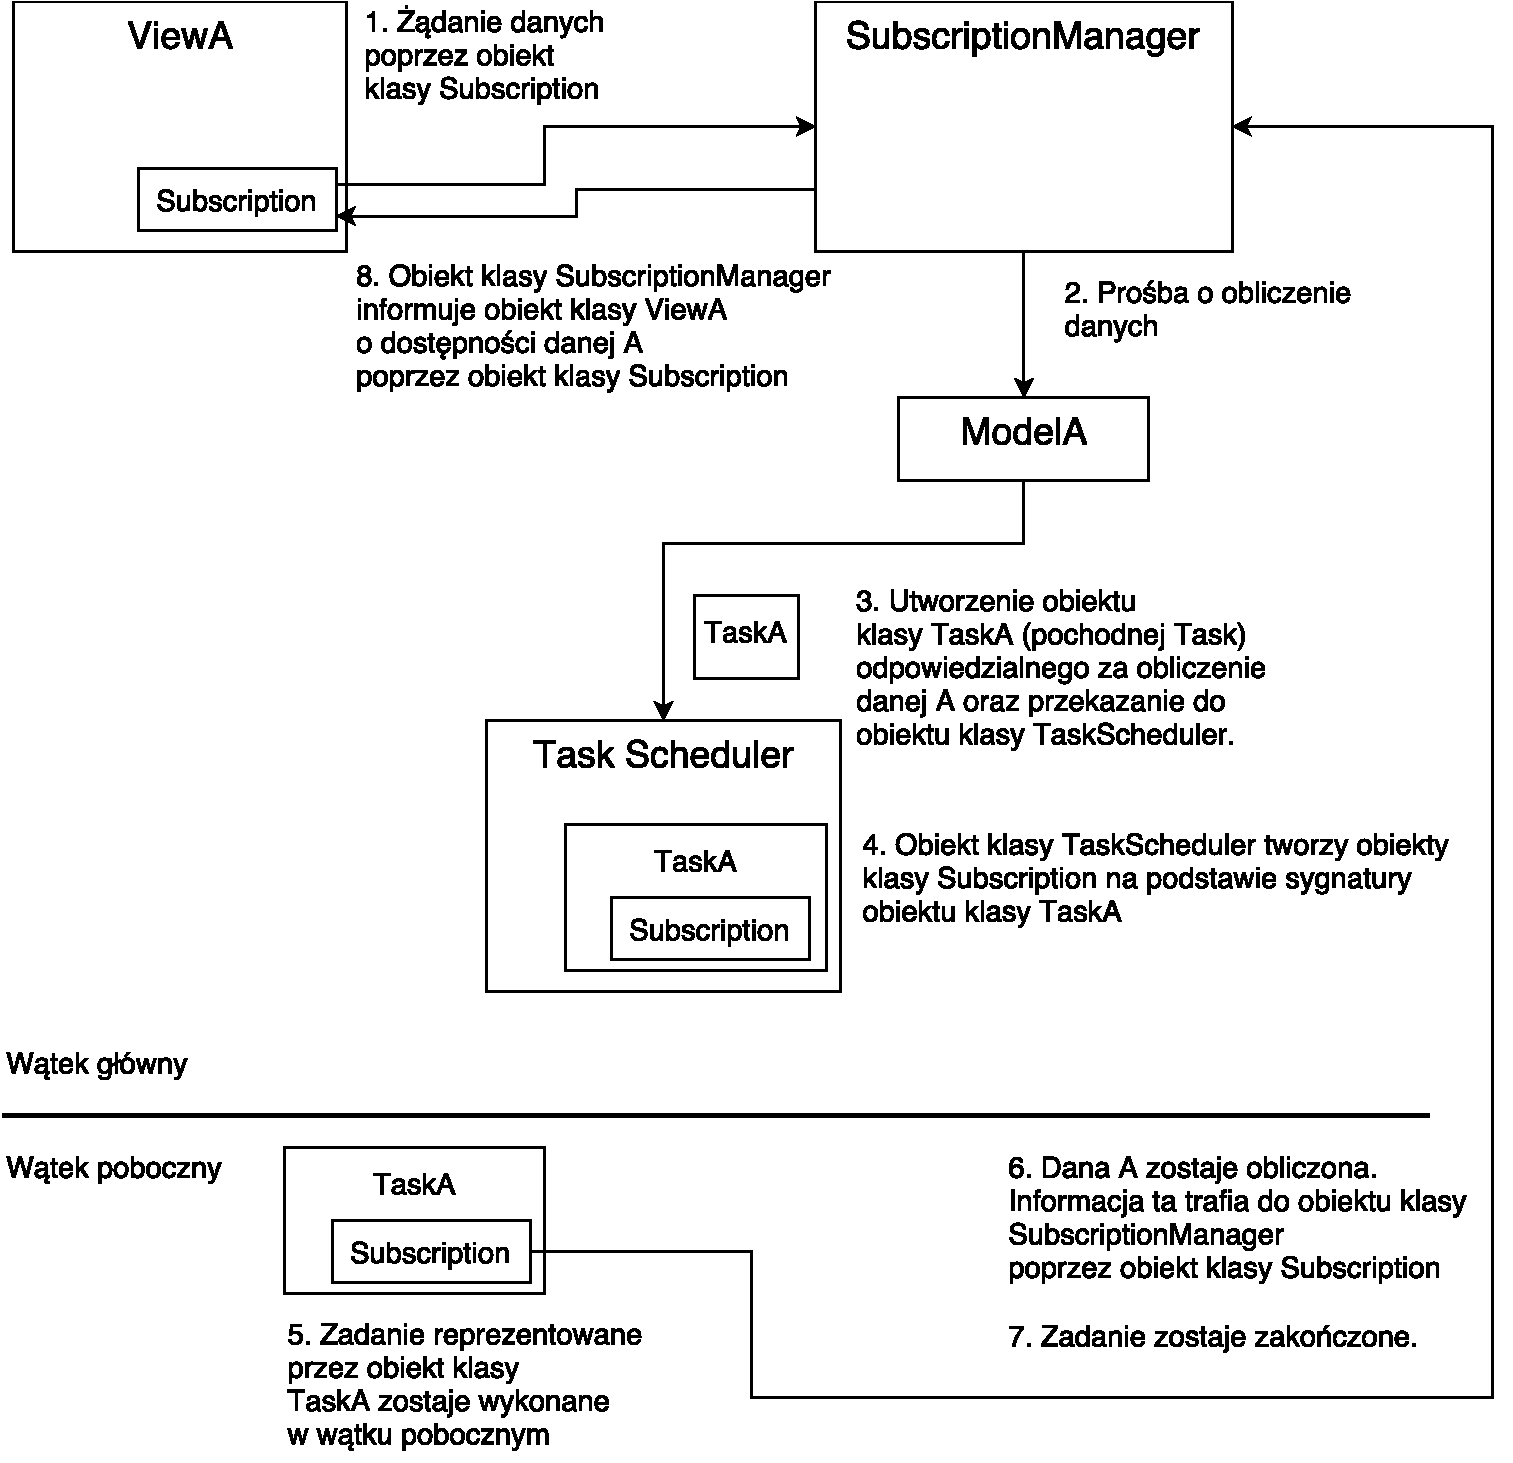
\includegraphics[width=0.6\linewidth]{rys05/scenario_1}
		\caption{Scenariusz przedstawiający żądanie obliczenia danej~A poprzez aktywowanie widoku~A (obiektu klasy \lstinline$ViewA$).}
		\label{fig:scenario1}	
	\end{figure}

	\begin{figure}[ht]
		\centering
		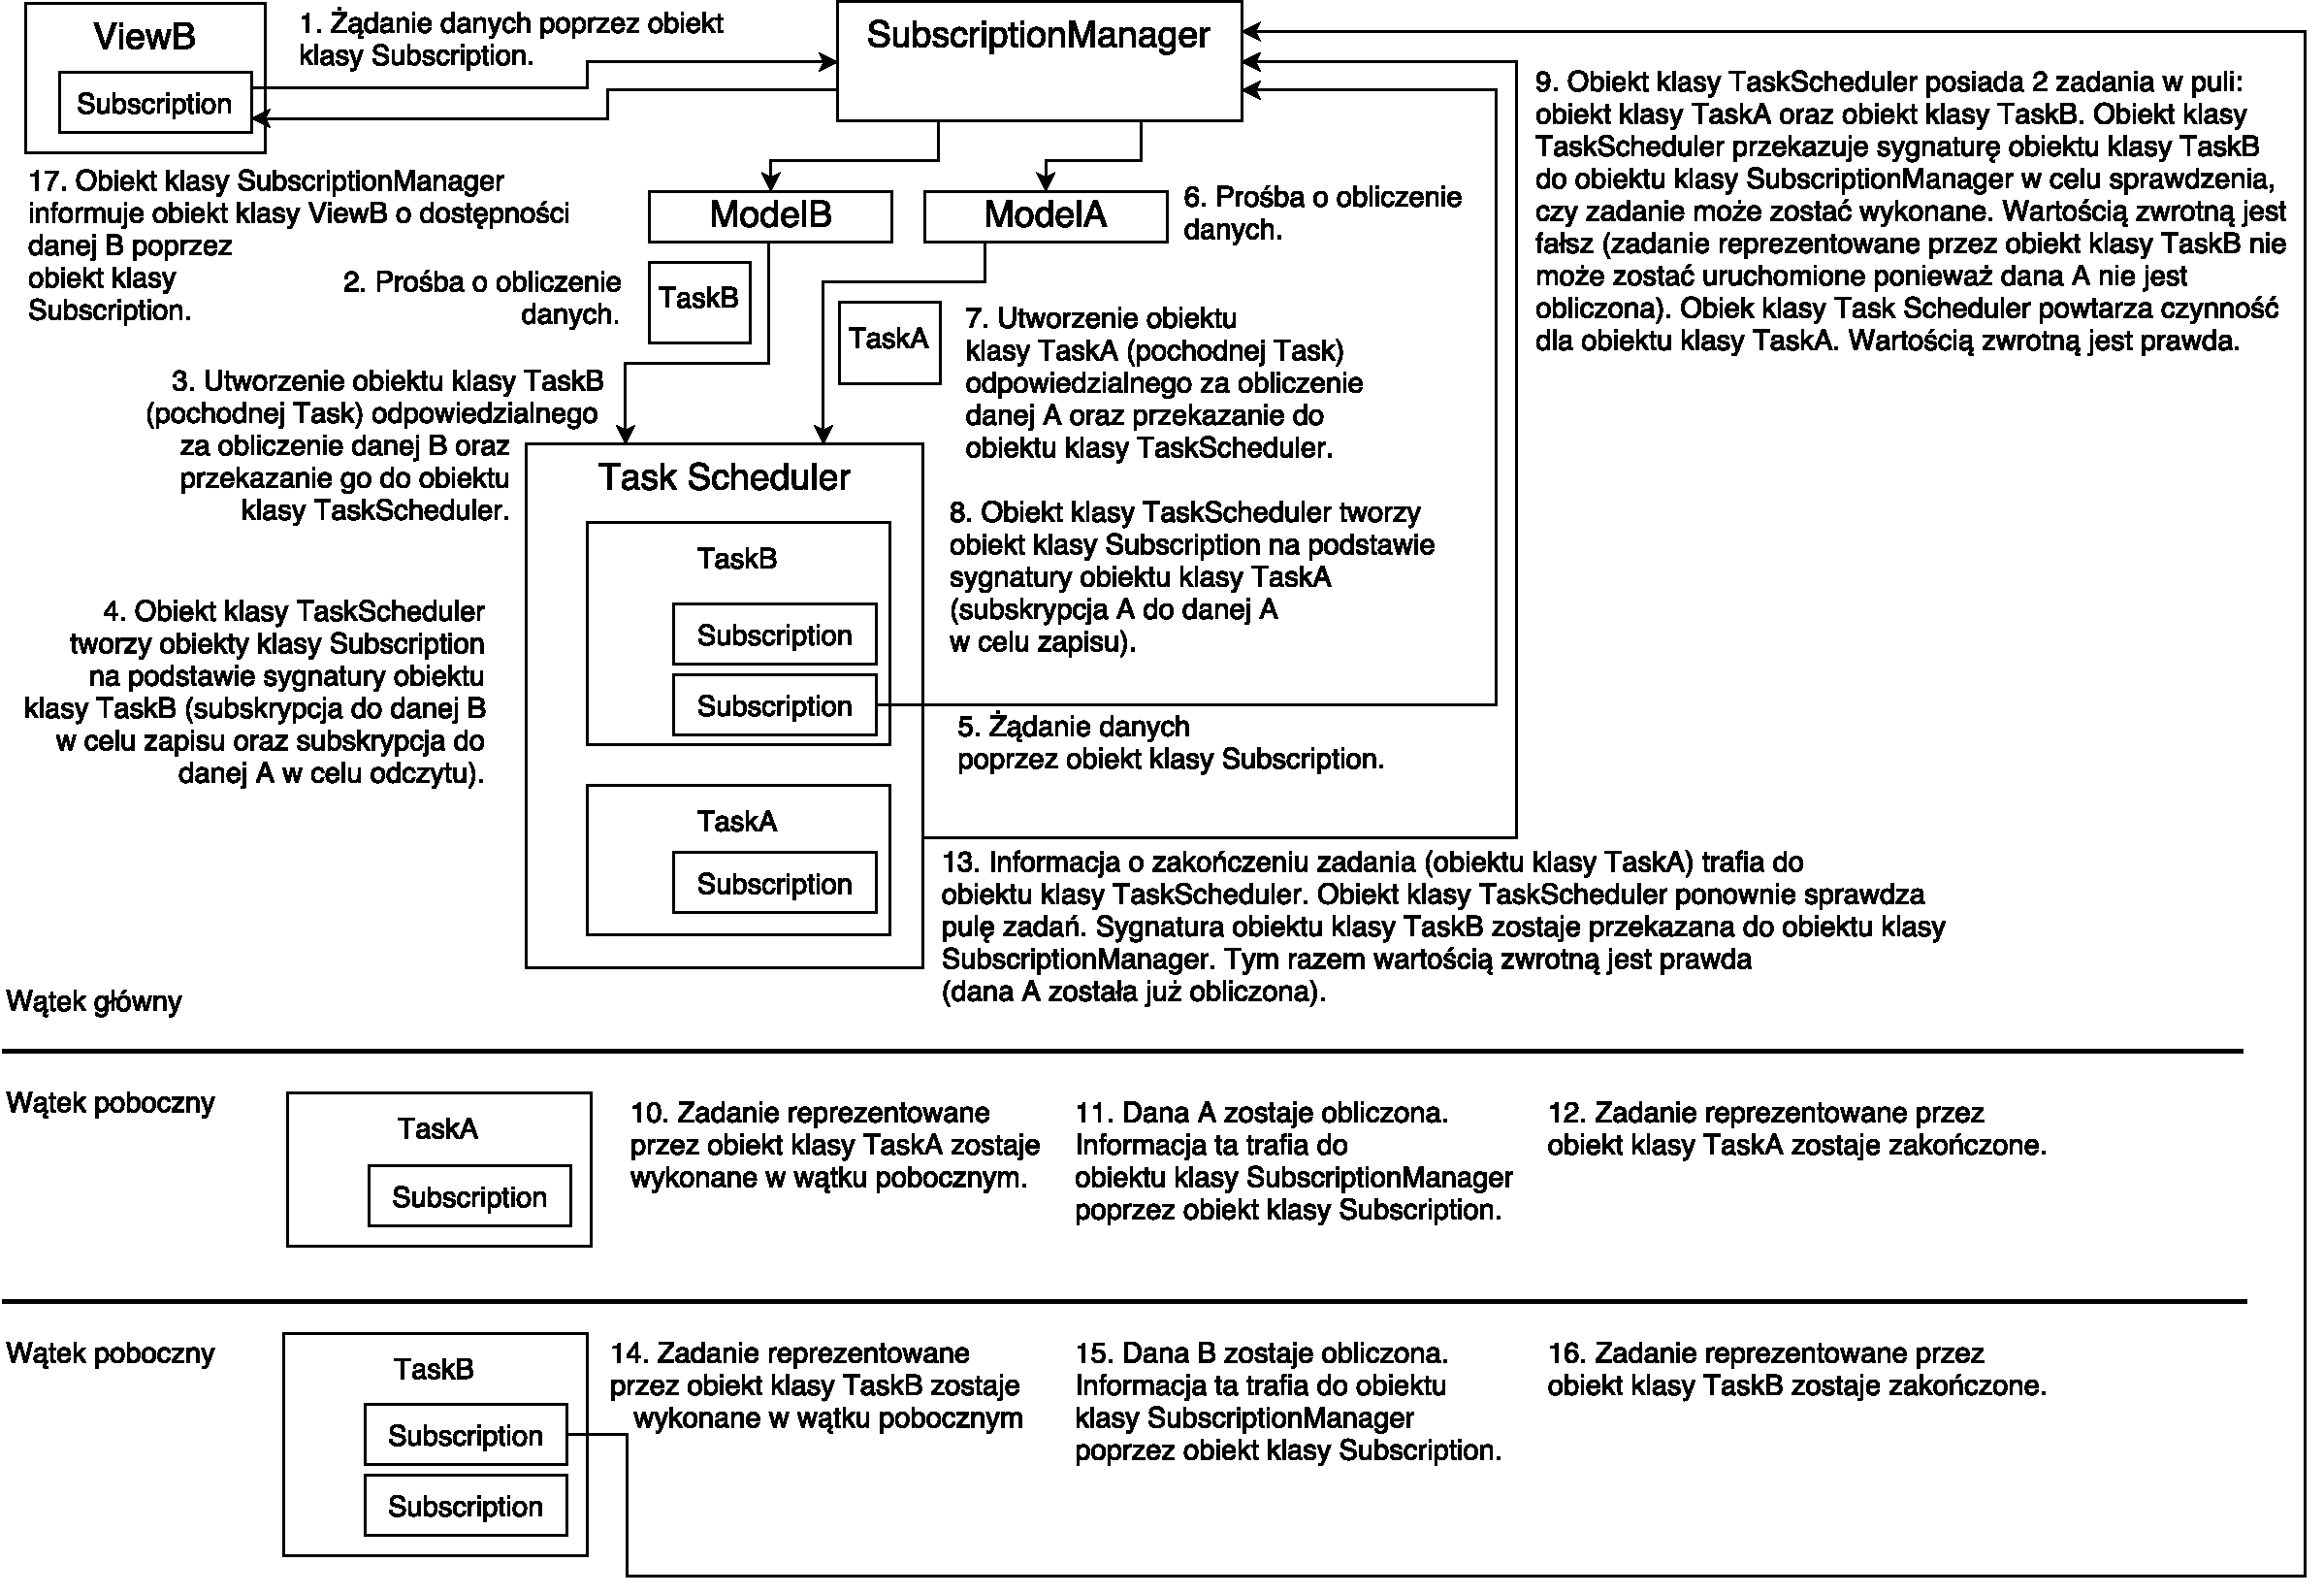
\includegraphics[width=0.8\linewidth]{rys05/scenario_2}
		\caption{Scenariusz przedstawiający żądanie obliczenia danej~B poprzez aktywowanie widoku~B (obiektu klasy \lstinline$ViewB$). Założenie początkowe: dana~B jest zależna od danej~A.}
		\label{fig:scenario2}	
	\end{figure}
	
	\begin{figure}[ht]
		\centering
		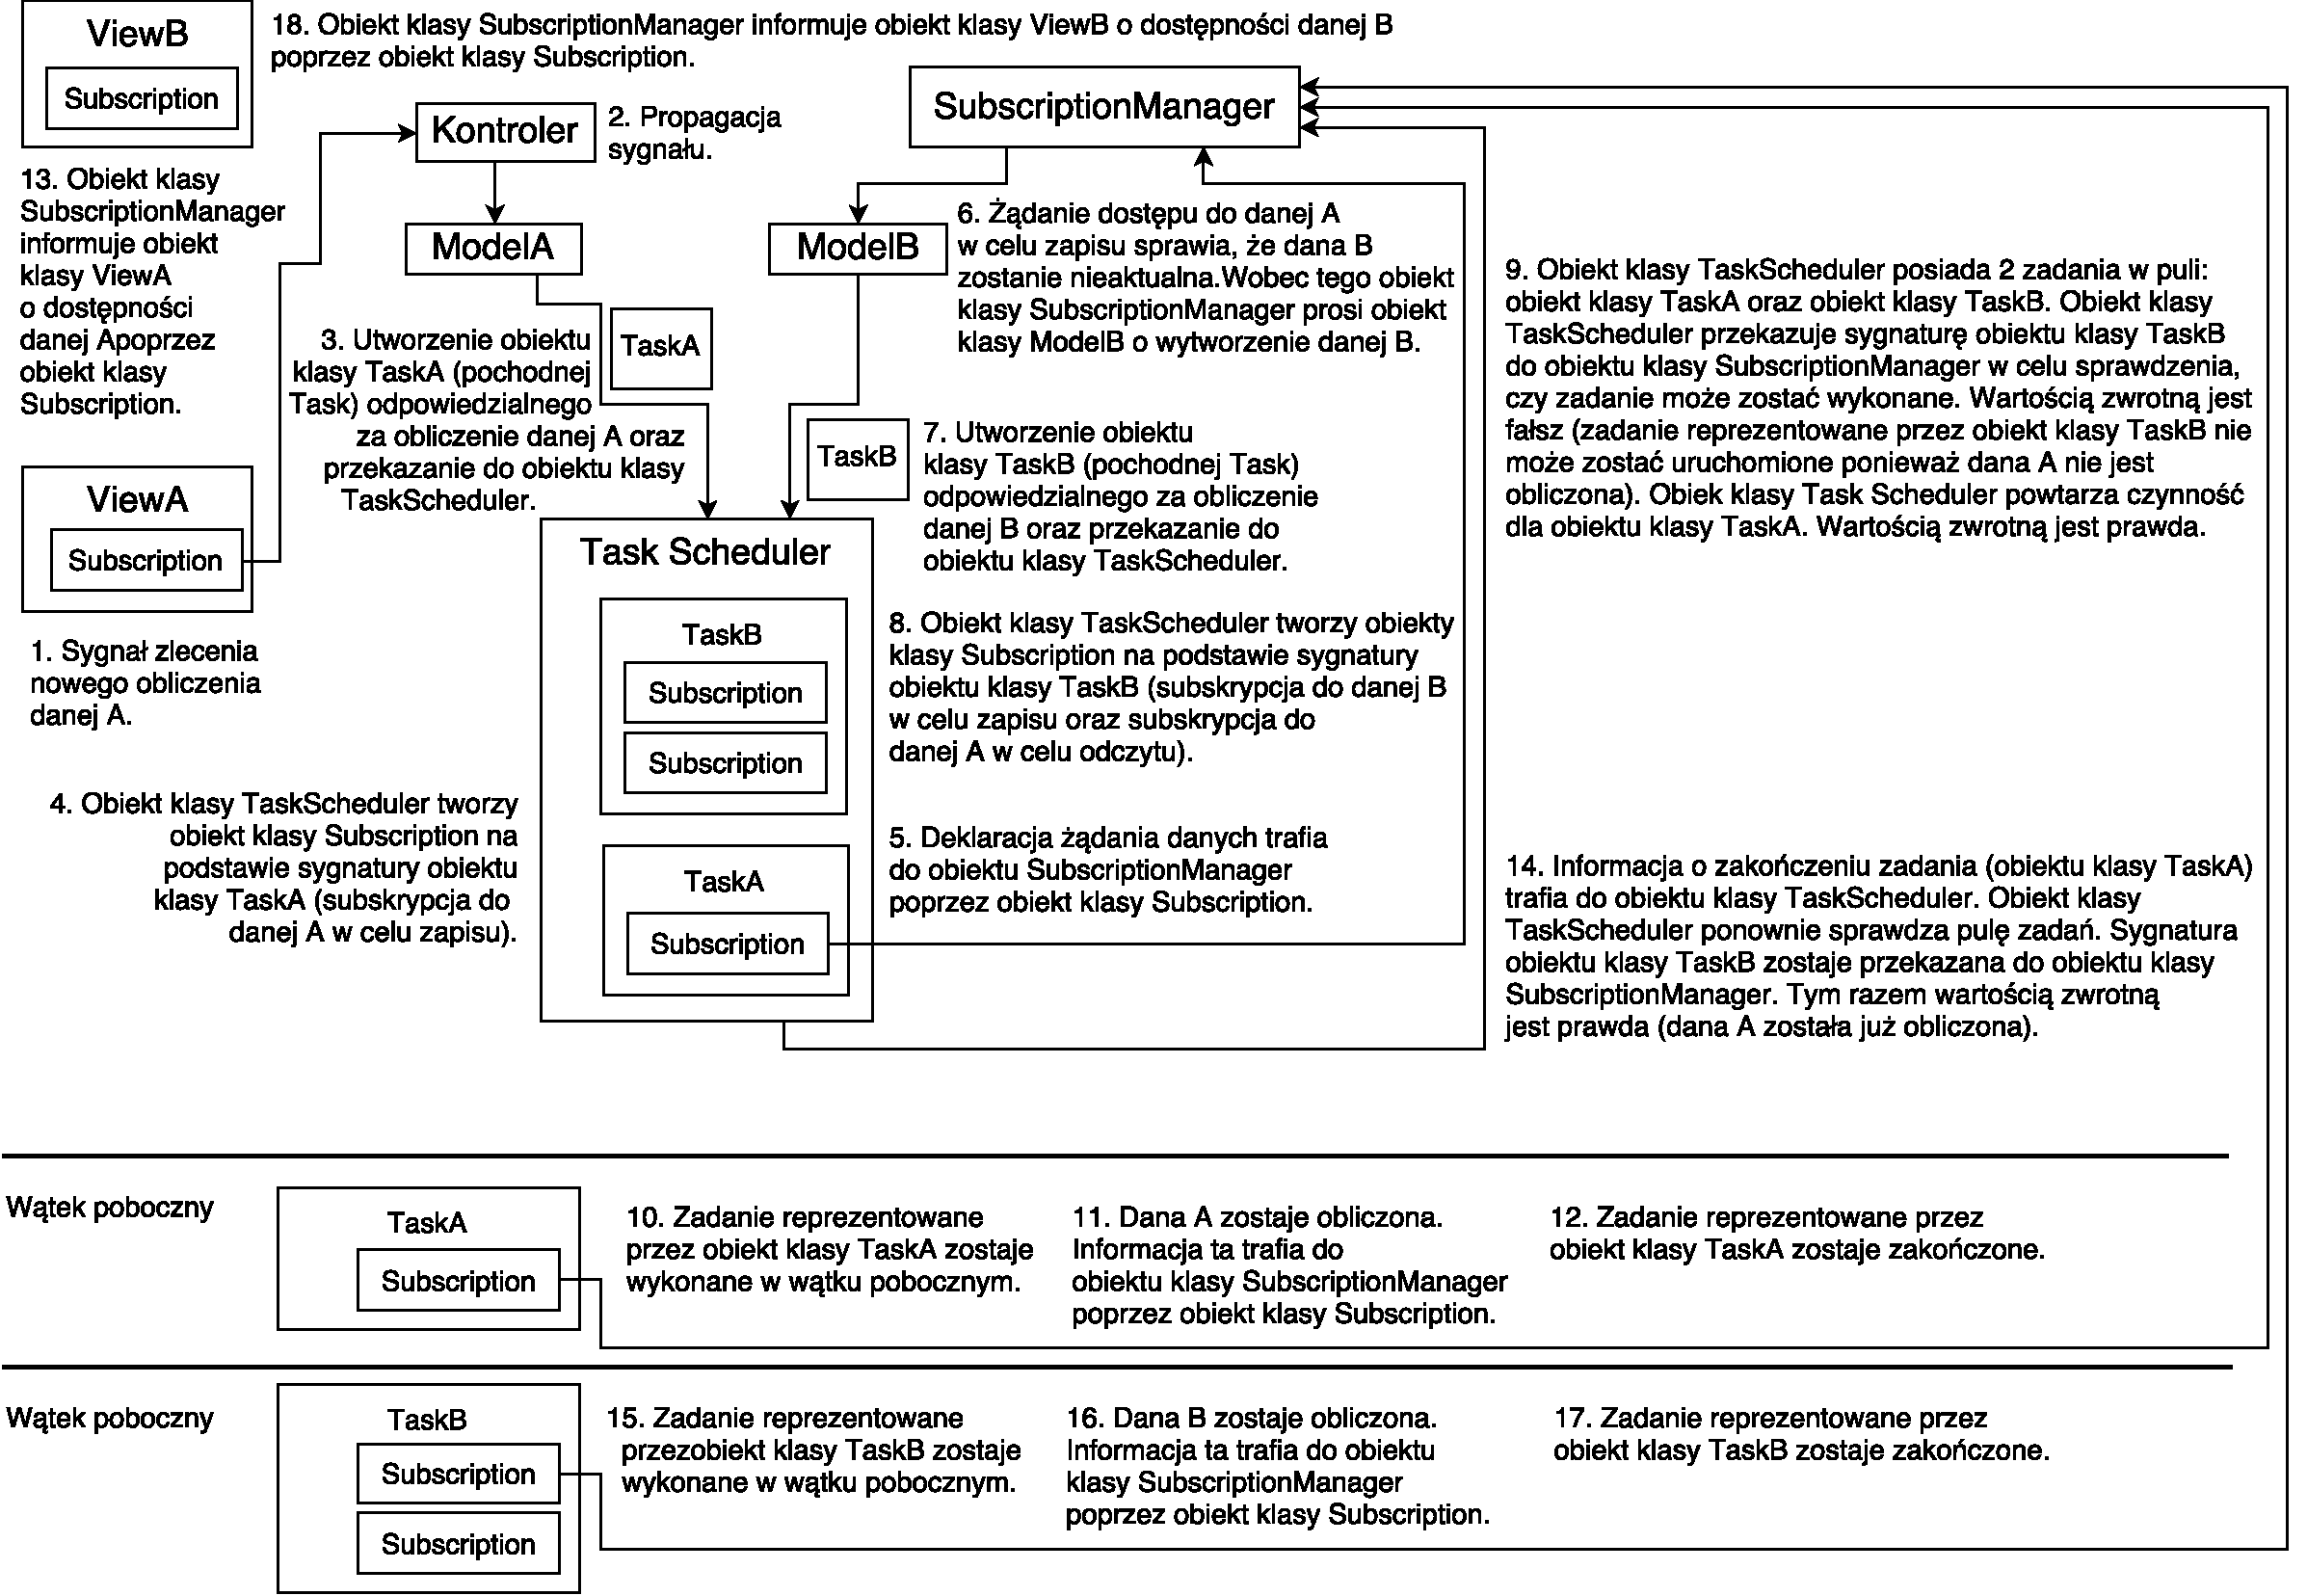
\includegraphics[width=0.8\linewidth]{rys05/scenario_3}
		\caption{Scenariusz przedstawiający żądanie obliczenia danej~A~poprzez interakcję użytkownika z~widokiem~A~(obiektem klasy \lstinline$ViewA$). Założenia początkowe: widoki~A~i~B są aktywne i~prezentują dane A~i~B. Dana~B jest zależna od danej~A.}
		\label{fig:scenario3}	
	\end{figure}

\end{landscape}

%\subsection{Streszczenie przepływu danych w systemie} % TUTAJ ZDECYDOWAĆ SIĘ NA JEDNO ALBO DRUGIE (TO ALBO TO POWYŻEJ)
%
%Obliczenia danych są wywoływane poprzez interakcję użytkownika z interfejsem graficznym. Dane są wizualizowane w konkretnych panelach. W celu prezentacji danych użytkownik musi aktywować dany panel. Z punktu widzenia systemu panel jest komponentem żądającym dostępu do danej w celu odczytu. W kodzie widoku tworzony jest obiekt klasy Subscription, który stanowi definicję takiego żądania. Obiekty tego typu stanowią interfejs pomiędzy komponentami żądającymi dostępu do danych a obiektem klasy SubscriptionManager. Jeżeli dane są aktualne, panel otrzymuje stosowną informację. W ciele metody obsługującej tę informację dokonywany jest faktyczny dostęp do danych, dzięki czemu dana zostaje zaprezentowana w GUI. Możliwy jest również scenariusz, w którym żądana dana nie jest aktualna, bądź nie została jeszcze zainicjalizowana. Wówczas system wysyła informację do odpowiedniego komponentu typu Model, który zadeklarował umiejętność wytworzenia tej danej. Komponent w odpowiedzi na informację tworzy obiekt klasy Task oraz przekazuje go do obiektu klasy TaskScheduler. Każdy obiekt zadania posiada pewne zależności wobec danych. Minimum stanowi żądanie dostępu do danej, która ma zostać obliczona, w celu zapisu. Zazwyczaj zależności dopełniają żądania dostępu do odczytu danych, od których obliczana dana zależy (o ile zależy). Obiekt klasy TaskScheduler tworzy odpowiednie obiekty subskrypcji dla danego zadania, na podstawie jego sygnatury zależności. Akcja ta może prowadzić do powstania kolejnych obiektów zadań (jeżeli zadanie żąda dostępu do danej, która również nie jest aktualna). Obiekt klasy TaskScheduler uruchamia powstałe zadania w osobnych wątkach. W momencie gdy dana zażądana przez użytkownika zostanie finalnie obliczona, panel GUI otrzymuje stosowną informację i może dokonać jej prezentacji.


\section{Model danych współdzielonych}
Ważne jest aby do roli danej współdzielonej można było promować każdą daną w~systemie. Dlatego model danej współdzielonej nie może opierać się na interfejsie, który inne klasy by implementowały, lecz na opakowaniu, w~które można każdą daną włożyć. Klasa danych współdzielonych nazwana została \lstinline$DataEntry$.

\subsection{Przechowywanie danych}
Kwestię przechowania dowolnego typu można rozwiązać poprzez wykorzystanie \lstinline$boost::any$. Natomiast problem uchwytu do danych, którego można użyć w~różnych fragmentach kodu rozwiązuje \lstinline$std::shared_ptr$. Z~tego powodu \lstinline$std::shared_ptr<boost::any>$ stanowi trzon modelu danych współdzielonych. Zarówno dane jak i~towarzyszące im metadane są przechowywane w~ten sposób. 
 
\begin{minipage}{\textwidth}
	\begin{lstlisting}[label=dataentry:alias, caption={Aliasy używane w~kodzie aplikacji.},alsoletter={()[].=}]
using handle = std::shared_ptr<boost::any>;
using handle_pair = std::tuple<handle, handle>;
	\end{lstlisting}
\end{minipage}

Aby kod był bardziej zwięzły stosowane są w~nim aliasy (Listing \ref{dataentry:alias}). Pierwsza linia jest skróceniem zapisu typu uchwytu do danych, natomiast druga skraca zapis pary takich uchwytów (para uchwytów często jest wykorzystywana do reprezentacji danych zagregowanych z~metadanymi).

\subsection{Synchronizacja dostępu do danych}
Rozwiązanie to jednak nie likwiduje problemu synchronizacji dostępu do danych. Wobec tego model został wzbogacony o~muteks oraz dwie zmienne warunkowe (Listing \ref{dataentry:sync}). Pierwsza zmienna warunkowa -- \lstinline$not_reading$ służy do obsłużenia wątków oczekujących na dostęp do danych w~celu zapisu, natomiast druga \lstinline$not_writing$ do obsługi wątków oczekujących na dostęp do danych w~celu odczytu.

\begin{minipage}{\textwidth}
	\begin{lstlisting}[label=dataentry:sync, caption={Składowe klasy \lstinline$DataEntry$ zapewniające bezpieczne użycie w~środowisku wielowątkowym.},alsoletter={()[].=}]
std::mutex mu;
std::condition_variable not_reading;
std::condition_variable not_writing;
	\end{lstlisting}
\end{minipage}

Z pomocą tych narzędzi model udostępnia metody pozwalające na bezpieczny dostęp do danych w~aplikacji wielowątkowej.

\begin{minipage}{\textwidth}
	\begin{lstlisting}[label=dataentry:sync:read, caption={Metody klasy \lstinline$DataEntry$ zapewniające bezpieczny odczyt danych współdzielonych w~środowisku wielowątkowym.},alsoletter={()[].=}]
handle_pair DataEntry::read()
{
	std::unique_lock<std::mutex> lock(mu);
	not_writing.wait(lock, [this]() {
		return !doWrite && initialized;
	});
	return handle_pair(data_handle, meta_handle);
}

void DataEntry::endRead()
{
	if (doReads == 0) not_reading.notify_one();
}
	\end{lstlisting}
\end{minipage}

Na listingu \ref{dataentry:sync:read} widoczna jest implementacja metod realizujących dostęp do danych w~celu odczytu. 

W metodzie \lstinline$read$ tworzona jest blokada, która zajmuje muteks. Następnie wątek wywołujący metodę zostaje uśpiony do momentu powiadomienia przez zmienną warunkową. Aby uniknąć fałszywych wybudzeń przekazywane jest dodatkowo wyrażenie lambda, która służy za predykat. Jeśli wartość zwrócona przez wyrażenie lambda jest prawdziwa (zawarte jest w~nim sprawdzenie czy wewnętrzny stan danej jest prawidłowy), wówczas wybudzenie jest słuszne. Po wybudzeniu zostaje zwrócona para uchwytów -- do danej oraz metadanej.

Metoda \lstinline$endRead$ służy do sygnalizacji zakończenia odczytu. W~jej ciele wykonywane jest sprawdzenie czy wewnętrzny stan danej jest prawidłowy. Jeśli jest, wówczas zmienna warunkowa \lstinline$not_reading$ dokonuje przebudzenia jednego z~wątków oczekujących na dostęp do danych w~celu zapisu.

\begin{minipage}{\textwidth}
	\begin{lstlisting}[label=dataentry:sync:write, caption={Metody klasy \lstinline$DataEntry$ zapewniające bezpieczny zapis danych współdzielonych w~środowisku wielowątkowym.},alsoletter={()[].=}]
handle_pair DataEntry::write()
{
	std::unique_lock<std::mutex> lock(mu);
	not_reading.wait(lock, [this]() {
		return doReads == 0 && !doWrite;
	});

	return handle_pair(data_handle, meta_handle);
}

void DataEntry::endWrite()
{
	if (!doWrite) not_writing.notify_all();
}
	\end{lstlisting}
\end{minipage}

Analizując implementację metod pozwalających na bezpieczny zapis danych przedstawionych na listingu \ref{dataentry:sync:write} można dostrzec dużą analogie do metod z~listingu \ref{dataentry:sync:read}. Jedyną zasadniczą różnicą jest fakt, że po zakończeniu zapisu zmienna warunkowa \lstinline$not_writing$ budzi wszystkie wątki oczekujące na dostęp w~celu odczytu.

\section{Klasa Model}

Model jest zmodyfikowaną wersją modelu z~wzorca MVC. Jego zadaniem jest kontrola procesu wytworzenia danej. Interfejs zdefiniowany dla modelu został przedstawiony na listingu \ref{modelInterface}.

\begin{minipage}{\textwidth}
	\begin{lstlisting}[label=modelInterface, caption={Interfejs klasy \lstinline$Model$.},alsoletter={()[].=}]
class Model : public QObject
{
	Q_OBJECT
public:
	explicit Model(SubscriptionManager& sm, TaskScheduler* scheduler,
						QObject *parent = 0);
	virtual ~Model();

public slots:
	virtual void delegateTask(QString requestedId,
								QString parentId = "") = 0;
	void taskFinished(QString id, bool success);

protected:
	void registerData(QString dataId,
						std::vector<QString> dependencies);
	bool isTaskCurrent(QString id);

private:
	SubscriptionManager& sm;
	TaskScheduler* scheduler;
	
	std::map<QString, std::shared_ptr<Task>> tasks;

};
	\end{lstlisting}
\end{minipage}


Metoda \lstinline$registerData$ służy do rejestrowania danych. Za jej pomocą model zgłasza współdzielone dane, za które bierze odpowiedzialność. Każda dana współdzielona, aby istnieć w~systemie, musi zostać zarejestrowana przez któryś z modeli (obiekt klasy pochodnej od klasy \lstinline$Model$). Do zarejestrowania danej wymagane jest jej identyfikator (ID) oraz lista ID danych, od której owa dana jest zależna. Na listingu \ref{model:registerData} został przedstawiony przykład rejestrowania współdzielonych danych. W~pierwszych dwóch liniach zarejestrowane zostały dane, które są niezależne (lista ich zależności jest pusta). W~trzeciej linii jest wyrażona rejestracja danej \lstinline$image.IMG$ oraz jej zależności od danych \lstinline$image$ oraz \lstinline$ROI$. Dzięki takiemu formatowi rejestrowania danych system jest w~stanie stworzyć graf zależności danych, wykorzystywany do prawidłowej propagacji informacji.

\begin{minipage}{\textwidth}
	\begin{lstlisting}[label=model:registerData, caption={Przykłady rejestrowania danych.},alsoletter={()[].=}]
registerData("image", {});
registerData("ROI", {});
registerData("image.IMG", {"image", "ROI"});
	\end{lstlisting}
\end{minipage}

Z analizy listingu \ref{modelInterface} wynika, że klasa implementująca interfejs \lstinline$Model$ musi zdefiniować metodę \lstinline$delegateTask$, aby nie być klasą abstrakcyjną. Metoda ta jest kluczowa dla tego interfejsu, oraz bardzo ważna dla całego systemu. W~definicji tej metody powinna znaleźć się obsługa żądania dokonania obliczeń danych. Żądanie takie może płynąć bezpośrednio od użytkownika, bądź w~sposób pośredni, na skutek wewnętrznego mechanizmu systemu. Standardowym zachowaniem modelu jest utworzenie odpowiedniego obiektu klasy implementującej interfejs \lstinline$Task$ i~przekazanie go do obiektu klasy \lstinline$TaskScheduler$. Teoretycznie możliwe jest, aby model sam dokonał obliczenia danej, zamiast tworzyć obiekt klasy implementującej interfejs \lstinline$Task$. Ta metoda jednak nie jest zalecana. Dopuszcza się jej stosowanie jedynie w~przypadku nieskomplikowanych obliczeń na małych strukturach danych. 

Dodatkowo na uwagę zasługuje metoda \lstinline$isTaskCurrent$, dzięki której można sprawdzić, czy istnieje aktualnie zadanie o~danym ID, oczekujące na wykonanie, bądź aktualnie wykonywane. Informacja ta jest pomocna w~tworzeniu rozbudowanej logiki modelu.

\section{Klasa Subscription oraz klasa Lock}
Obiekt klasy \lstinline$Subscription$ pełni rolę pośrednika między jednostką zarządzającą danymi a~jednostką, która o~dostęp do danych prosi. Poprzez utworzenie obiektu klasy \lstinline$Subscription$ komponent deklaruje chęć uzyskania dostępu do konkretnej danej (utworzenie subskrypcji do danej). Do stworzenia takiego obiektu potrzebne jest ustalenie jego przeznaczenia (odczyt bądź zapis) oraz podanie nazwy pożądanej danej.
 
Aby dokonać faktycznego dostępu do danej tworzy się obiekt klasy \lstinline$Lock$. Podczas inicjalizacji przekazuje mu się obiekt klasy \lstinline$Subscription$. \lstinline$Lock$ jest szablonem klasy. Podczas tworzenia takiego obiektu należy skonkretyzować go dwoma typami: pierwszy jest typem żądanej danej, natomiast drugi jest typem jej metadanej. Jeżeli jednak nie ma się zamiaru korzystać z~metadanej, nie ma potrzeby podawania jej typu. Za pomocą obiektu klasy \lstinline$Lock$ można otrzymać bezpośredni uchwyt do danej oraz do metadanej. Podczas pozyskiwania uchwytów wewnętrzna implementacja klasy \lstinline$Lock$ dokonuje rzutowania z~typu \lstinline$boost::any$ na podany przy tworzeniu obiektu klasy \lstinline$Lock$ typ, stąd potrzeba ich specyfikowania. Dostęp do danych może być blokujący -- wykonanie w~wątku dokonującym dostępu do danych może zostać wstrzymane. Wynika to z~mechanizmów odczytu/zapisu modelu danych współdzielonych oraz logiki jednostki zarządzającej danymi.

Klasa \lstinline$Subscription$ zapewnia jeszcze jedną bardzo ważną funkcjonalność. Jest nią sygnalizowanie aktualizacji danych. Jest to bardzo przydatne dla komponentów interfejsu graficznego, których zadaniem jest prezentowanie żądanych danych oraz dbanie o~aktualność tych danych. Aby ułatwić to zadanie, komponent GUI może podczas tworzenia obiektu klasy \lstinline$Subscription$ przekazać metodę, w~ciele której realizowana będzie obsługa sygnału aktualizacji danej. Dzięki temu komponenty takie jak widok nie muszą posiadać logiki sprawdzania czy dane zostały zaktualizowane. Taki sposób dostępu do danych został nazwany odroczonym (ang. deferred). Konstrukcja obiektu klasy \lstinline$Subscription$ w~ten sposób została przedstawiona na listingu \ref{subscription:deferred}. W~opozycji do dostępu odroczonego stoi dostęp bezpośredni (ang. direct), który jest bardziej uniwersalny. Jest to nic innego jak utworzenie obiektu klasy \lstinline$Subscription$ oraz obiektu klasy \lstinline$Lock$. Deklarując dostęp odroczony przy tworzeniu obiektu subskrypcji można używać również dostępu bezpośredniego (co zazwyczaj ma miejsce w~ciele metody, która jest obsługą sygnału aktualizacji danej). Nie można jednak używać dostępu odroczonego jeśli obiekt klasy \lstinline$Subscription$ został utworzony z~zadeklarowanym dostępem bezpośrednim. Konstrukcja dostępu bezpośredniego została przedstawiona na listingu \ref{subscription:direct}.

\begin{minipage}{\textwidth}
	\begin{lstlisting}[label=subscription:deferred, caption={Przykład tworzenia obiektu klasy \lstinline$Subscription$ z~odroczonym dostępem do danych.},alsoletter={()[].=}]	
Subscription* sub = SubscriptionFactory::create(Dependency("image.IMG",
	SubscriptionType::READ), AccessType::DEFERRED, this,
	std::bind(&ImgWindow::displayImg, this));
	
	
	\end{lstlisting}
\end{minipage}

\begin{minipage}{\textwidth}
	\begin{lstlisting}[label=subscription:direct, caption={Przykład tworzenia obiektu klasy \lstinline$Subscription$ z~bezpośrednim dostępem do danych.},alsoletter={()[].=}]
Subscription* sub = SubscriptionFactory::create(Dependency("image.IMG",
	SubscriptionType::READ), AccessType::DIRECT);
	
	\end{lstlisting}
\end{minipage}

Aby umożliwiać dostęp do danych, obiekt klasy \lstinline$Subscription$ potrzebuje uchwytu do jednostki zarządzającej danymi (obiektu klasy \lstinline$SubscriptionManager$). Ważne jest jednak, aby dostęp do danych współdzielonych był prosty dla wszystkich komponentów w~systemie -- również tych, które nie mają dostępu do jednostki zarządzania danymi. Zatem aby tworzenie obiektów klasy \lstinline$Subscription$ było możliwe z~dowolnego miejsca w~kodzie realizowane jest ono poprzez obiekt klasy \lstinline$SubscriptionFactory$. Klasa ta jest implementacją wzorca projektowego -- fabryki. Obiekt klasy \lstinline$SubscriptionFactory$ posiada uchwyt do obiektu klasy \lstinline$SubscriptionManager$, który przekazuje obiektowi klasy \lstinline$Subscription$ podczas jego inicjalizacji. 

\section{Klasa Task}
Klasa \lstinline$Task$ jest odpowiedzialna za bezpośrednie obliczenie danych. Służy zatem do zaktualizowania danej bądź jej inicjalizacji. Jest to klasa abstrakcyjna służąca jako interfejs. W~dalszej części tekstu obiekt klasy implementującej interfejs \lstinline$Task$ nazywany będzie obiektem zadania. Podstawową zasadą obiektu zadania jest to, że zawsze dokonuje on modyfikacji tylko jednej danej, natomiast może bazować na dowolnej liczbie danych, określanych jako "źródła". 

Każdy obiekt zadania posiada składową \lstinline$dependencies$, która jest listą jego zależności. Złożona jest ona z~danej modyfikowanej oraz źródeł. Dla każdej danej w~liście zależności określony jest również cel dostępu do niej (odczyt bądź zapis).

Identyfikator (ID) modyfikowanej danej musi zostać przekazany obiektowi zadania jako parametr jego konstruktora. Identyfikatory źródeł również są przekazywane w~konstruktorze, lecz w~postaci mapy. W~mapie tej kluczem jest identyfikator źródła, natomiast wartością identyfikator, według którego ta dana będzie rozróżniana wewnątrz zadania. Jest to zabieg zastosowany w~celu ujednolicenia konwencji nazewniczej wewnątrz obiektów zadań. Zazwyczaj obiekty te posiadają jedynie jedno źródło, do którego odnoszą się za pomocą identyfikatora \lstinline$source$. ID danej modyfikowanej jest automatycznie mapowany na nazwę \lstinline$dest$. 

Obiekty zadań, aby móc realizować dostęp do danych musi posiadać odpowiednie obiekty klasy \lstinline$Subscription$. Przeznaczona na nie jest składowa \lstinline$subscriptions$. Komponent nadrzędny, zarządzający zadaniem (obiekt klasy \lstinline$TaskScheduler$) jest zobowiązany do utworzenia dla niego właściwych obiektów klasy \lstinline$Subscription$ (na podstawie jego zależności, zwracanych przez metodę \lstinline$getDependencies$) oraz przekazania ich poprzez metodę \lstinline$setSubscription$. Teoretycznie obiekt zadania może sam tworzyć obiekty klasy \lstinline$Subscription$, jednak nie jest to zalecane, a~wręcz uznawane za błąd koncepcyjny. Jego przeznaczeniem jest dokonywanie obliczeń na danych. Komponent tego typu nie powinien zajmować się zarządzaniem obiektami klasy \lstinline$Subscription$.

Każdy obiekt zadania posiada własny identyfikator. Może być on przekazany jako parametr konstruktora. Jeżeli nie jest, wówczas identyfikatorem obiektu zadania staje się identyfikator modyfikowanej danej. Wywołanie metody \lstinline$start$ może być rozumiane jako uruchomienie obiektu zadania, natomiast jej zakończenie jako zakończenie wykonywania zadania. W~jej ciele dokonywana jest faktyczna kalkulacja danej.

Interfejs klasy \lstinline$Task$ został przedstawiony na listingu \ref{task:interface}. 

\begin{minipage}{\textwidth}
	\begin{lstlisting}[label=task:interface, caption={Interfejs klasy \lstinline$Task$.},alsoletter={()[].=}]
class Task : public QObject
{
	Q_OBJECT
public:
	explicit Task(QString target, std::map<QString, QString> sources);
	explicit Task(QString id, QString target, std::map<QString, QString> sources);

	virtual ~Task();
	virtual bool start() final;
	virtual void setSubscription(QString id, std::shared_ptr<Subscription> sub) final;

	std::vector<Dependency>& getDependencies();
	QString getId();

signals:
	void finished(QString id, bool success);

protected:
	virtual bool run() = 0;
	virtual std::shared_ptr<Subscription> sub(QString id) final;
	virtual bool subExists(QString id) final;
	virtual bool isCancelled();

private:
	QString id;
	std::vector<Dependency> dependencies;
	std::map<QString, QString> sources;
	std::map<QString, std::shared_ptr<Subscription>> subscriptions;

};
	\end{lstlisting}
\end{minipage}

Analizując listing \ref{task:interface} można ustalić, że klasy implementujące interfejs \lstinline$Task$ muszą zdefiniować metodę \lstinline$run$, aby nie być abstrakcyjne. Co więcej, wystarczające jest aby klasa zdefiniowała jedynie konstruktory oraz tę metodę, ponieważ właśnie ta ona przeznaczona jest do wykonywania obliczeń na danych. Wszelkie pozostałe metody mają charakter pomocniczy oraz są zapewnione przez klasę bazową. W~jej ciele do obiektu klasy \lstinline$Subscription$ można się odwołać za pomocą metody \lstinline$sub$. Można również sprawdzić czy obiekt klasy \lstinline$Subscription$ został utworzony dzięki metodzie \lstinline$subExists$. Argumentem obu tych metod jest wewnętrzny identyfikator danej. Obiekt zadania po zakończeniu metody \lstinline$run$ emituje sygnał \lstinline$finished$. Informacja taka może być przydatna dla modelu odpowiedzialnego za dane zadanie.

\section{Klasa TaskScheduler} 
Klasa \lstinline$TaskScheduler$ jest odpowiedzialna za zarządzanie obiektami zadań. W całym systemie powinna występować jedynie jedna instancja tej klasy. Wymaganie to implikuje pomysł wykorzystania wzorca projektowego singleton do implementacji tej klasy~\cite{singleton}. Jednak ten wzorzec projektowy nie został wykorzystany -- powodem jest trudność zarządzania singletonem, np. w przypadku wykonywania testów jednostkowych. Jak można wywnioskować z~listingu \ref{scheduler:interface} klasa ta nie jest skomplikowana. Poprzez jedyną publiczną metodę -- \lstinline$pushTask$ trafiają do niej obiekty zadań utworzone przez modele. Gdy obiekt taki zostanie przekazany do obiektu klasy \lstinline$TaskScheduler$, ten tworzy dla niego obiekty klasy \lstinline$Subscription$. Funkcjonalność tę realizuje metoda \lstinline$createSubscriptions$. Obiekt zadania, który posiada utworzone obiekty klasy \lstinline$Subscription$ trafia do puli zadań (składowa \lstinline$taskPool$). Po dodaniu obiektu zadania do puli, pula zostaje przeiterowana w~poszukiwaniu obiektów zadań gotowych do uruchomienia. Predykatem w~kwestii, czy obiekt zadania może zostać uruchomiony, czy też nie jest metoda \lstinline$processDependencies$ klasy \lstinline$SubscriptionManager$. Obiekt klasy \lstinline$TaskScheduler$ przekazuje mu listę zależności obiektu zadania, a~z powrotem otrzymuje wartość logiczną. Jeżeli jest ona równa \lstinline$true$, wówczas obiekt klasy \lstinline$TaskScheduler$ uruchamia obiekt zadania za pomocą metody \lstinline$startTask$. Jeżeli otrzymana wartość wynosi \lstinline$false$, obiekt klasy \lstinline$TaskScheduler$ nie podejmuje żadnych akcji dla tego obiektu zadania i~powraca do iteracji puli.

W metodzie \lstinline$startTask$ tworzony jest wątek, do którego przekazywany jest obiekt zadania. Wątek jest uruchamiany, a~w nim uruchamiany zostaje obiekt zadania. Dodatkowo ustanawiane jest połączenie, za pomocą którego po zakończeniu obiektu zadania obiekt klasy \lstinline$TaskScheduler$ ponownie iteruje pulę zadań w~celu znalezienia kandydata do uruchomienia. 

\begin{minipage}{\textwidth}
	\begin{lstlisting}[label=scheduler:interface, caption={Deklaracja klasy \lstinline$TaskScheduler$.},alsoletter={()[].=}]
class TaskScheduler : public QObject
{
	Q_OBJECT
public:
	TaskScheduler(SubscriptionManager& sm);
	void pushTask(std::shared_ptr<Task> task);

private:
	void checkTaskPool();
	void startTask(std::shared_ptr<Task> task);
	void createSubscriptions(std::shared_ptr<Task> task);

	std::list<std::shared_ptr<Task>> taskPool;
	SubscriptionManager& sm;
};
	\end{lstlisting}
\end{minipage}

\section{Klasa SubscriptionManager}
Klasa \lstinline$SubscriptionManager$ pełni rolę głównego komponentu systemu. W~całym systemie powinna występować jedynie jedna instancja klasy \lstinline$SubscriptionManager$. Podobnie jak typ \lstinline$TaskScheduler$, typ \lstinline$SubscriptionManager$ to kandydat do wykorzystania wzorca projektowego singleton. Nie został on jednak użyty z identycznych powodów jak w przypadku klasy \lstinline$TaskScheduler$. Obiekt tej klasy agreguje wszystkie dane współdzielone oraz nimi zarządza. Do jego odpowiedzialności należą:
\begin{itemize}
	\item przyznawanie dostępu do danych,
	\item propagacja informacji o~dostępności nowej wersji danych,
	\item propagacja informacji o~żądaniu obliczeń nowych danych,
	\item zarządzanie cyklem życia danych,
	\item kontrola wewnętrznego stanu danych.
\end{itemize}

Funkcjonalności oferowane przez omówione wcześniej komponenty -- obiekty klasy \lstinline$Subscription$ oraz obiekty klasy \lstinline$Lock$ nie są przez nie realizowane. Klasa \lstinline$Subscription$ czy klasa \lstinline$Lock$ stanowi jedynie interfejs udostępniający funkcjonalności klasy \lstinline$SubscriptionManager$. Dla każdej danej kontrolowanej przez obiekt tej klasy przechowywane są następujące informacje:
\begin{itemize}
	\item liczba obiektów klasy \lstinline$Subscription$ utworzonych w~celu odczytu danej,
	\item flaga wskazująca na istnienie obiektu klasy \lstinline$Subscription$ utworzonego w~celu zapisu danej,
	\item liczba aktywnych dostępów do danych w~celu odczytu - pierwsza próba dostępu do danej bądź metadanej przy użyciu obiektu klasy \lstinline$Lock$ jest rejestrowana przez obiekt klasy \lstinline$SubscriptionManager$ jako aktywny dostęp do danych. Dostęp jest uznawany za zakończony gdy obiekt klasy \lstinline$Lock$ wyjdzie poza zasięg, bądź przez jawne zakończenie dostępu poprzez metodę \lstinline$release$ klasy \lstinline$Lock$,
	\item flaga wskazująca na aktywny dostęp do danych w~celu zapisu - analogicznie jak w~przypadku powyższym,
	\item flaga determinująca czy dana została zainicjalizowana,
	\item flaga determinująca czy dana jest aktualna,
	\item uchwyt do modelu, który zarejestrował daną,
	\item kolekcję identyfikatorów danych zależnych,
	\item kolekcję obiektów klasy \lstinline$Subscription$ utworzonych w~celu dostępu do tej danej.
\end{itemize}

Gdy jakiś komponent utworzy obiekt klasy \lstinline$Subscription$, obiekt ten staje się pośrednikiem w~celu dostępu do danej pomiędzy danym komponentem, a~obiektem klasy \lstinline$SubscriptionManager$. 

Jeśli obiekt klasy \lstinline$Subscription$ został stworzony w~celu odczytu danej, klasa \lstinline$SubscriptionManager$ inkrementuje liczbę takich obiektów. Jeżeli ze stanu danej wynika, że nie jest ona aktualna bądź zainicjalizowana obiekt klasy \lstinline$SubscriptionManager$ wysyła żądanie o~utworzenie zadania obliczającego do modelu odpowiedzialnego za tą daną. Jeżeli dana jest aktualna oraz nie odbywa się aktualnie zapis tej danej a~obiekt klasy \lstinline$Subscription$ został utworzony ze zdefiniowanym odroczonym sposobem dostępu do danej, obiekt klasy \lstinline$SubscriptionManager$ wysyła sygnał do komponentu (poprzez obiekt klasy \lstinline$Subscription$), mówiący że dana jest aktualna i~można przeprowadzić do niej dostęp. Scenariusz ten został przedstawiony na rysunku \ref{fig:subscribe}.

Jeśli obiekt klasy \lstinline$Subscription$ został stworzony w~celu zapisu (modyfikacji) danej, klasa \lstinline$SubscriptionManager$ przypisuje wartość logiczną prawdy do flagi wskazującej na obecność takiego typu obiektu oraz wartość logiczną fałszu do flagi wskazującej na aktualność danej. Następnie sygnał o~modyfikacji danej jest propagowany w~dół grafu zależności danych. Jeżeli któraś z~danych zależnych od danej, która będzie zmodyfikowana, jest bezpośrednio lub pośrednio subskrybowana (istnieją obiekty klasy \lstinline$Subscription$ utworzone w~celu dostępu do tej danej, bądź danej od niej zależnej), wówczas do modelu odpowiedzialnego za nią wysyłane jest żądanie o~utworzenie obiektu zadania obliczającego. Zazwyczaj model reaguje pozytywnie -- tworzy obiekt zadania, przekazuje go do obiektu klasy \lstinline$TaskScheduler$, który tworzy obiekty klasy \lstinline$Subscription$ dla obiektu zadania (w tym zawsze jeden w celu zapisu), przez co wykonanie znowu znajduje się w~punkcie rejestrowania faktu subskrypcji (utworzenia obiektu klasy \lstinline$Subscription$) przez klasę \lstinline$SubscriptionManager$, tym razem jednak dla danej pochodnej. Proces ten w~sposób rekurencyjny powtarza się dla wszystkich danych zależnych od wyjściowej danej. W~następnym kroku dla każdej danej zależnej od danej wyjściowej, fladze wskazującej na aktualność danej zostaje przypisana wartość logiczna fałszu. Scenariusz ten został przedstawiony na rysunku \ref{fig:subscribe}.

\begin{figure}[ht]
	\centering
	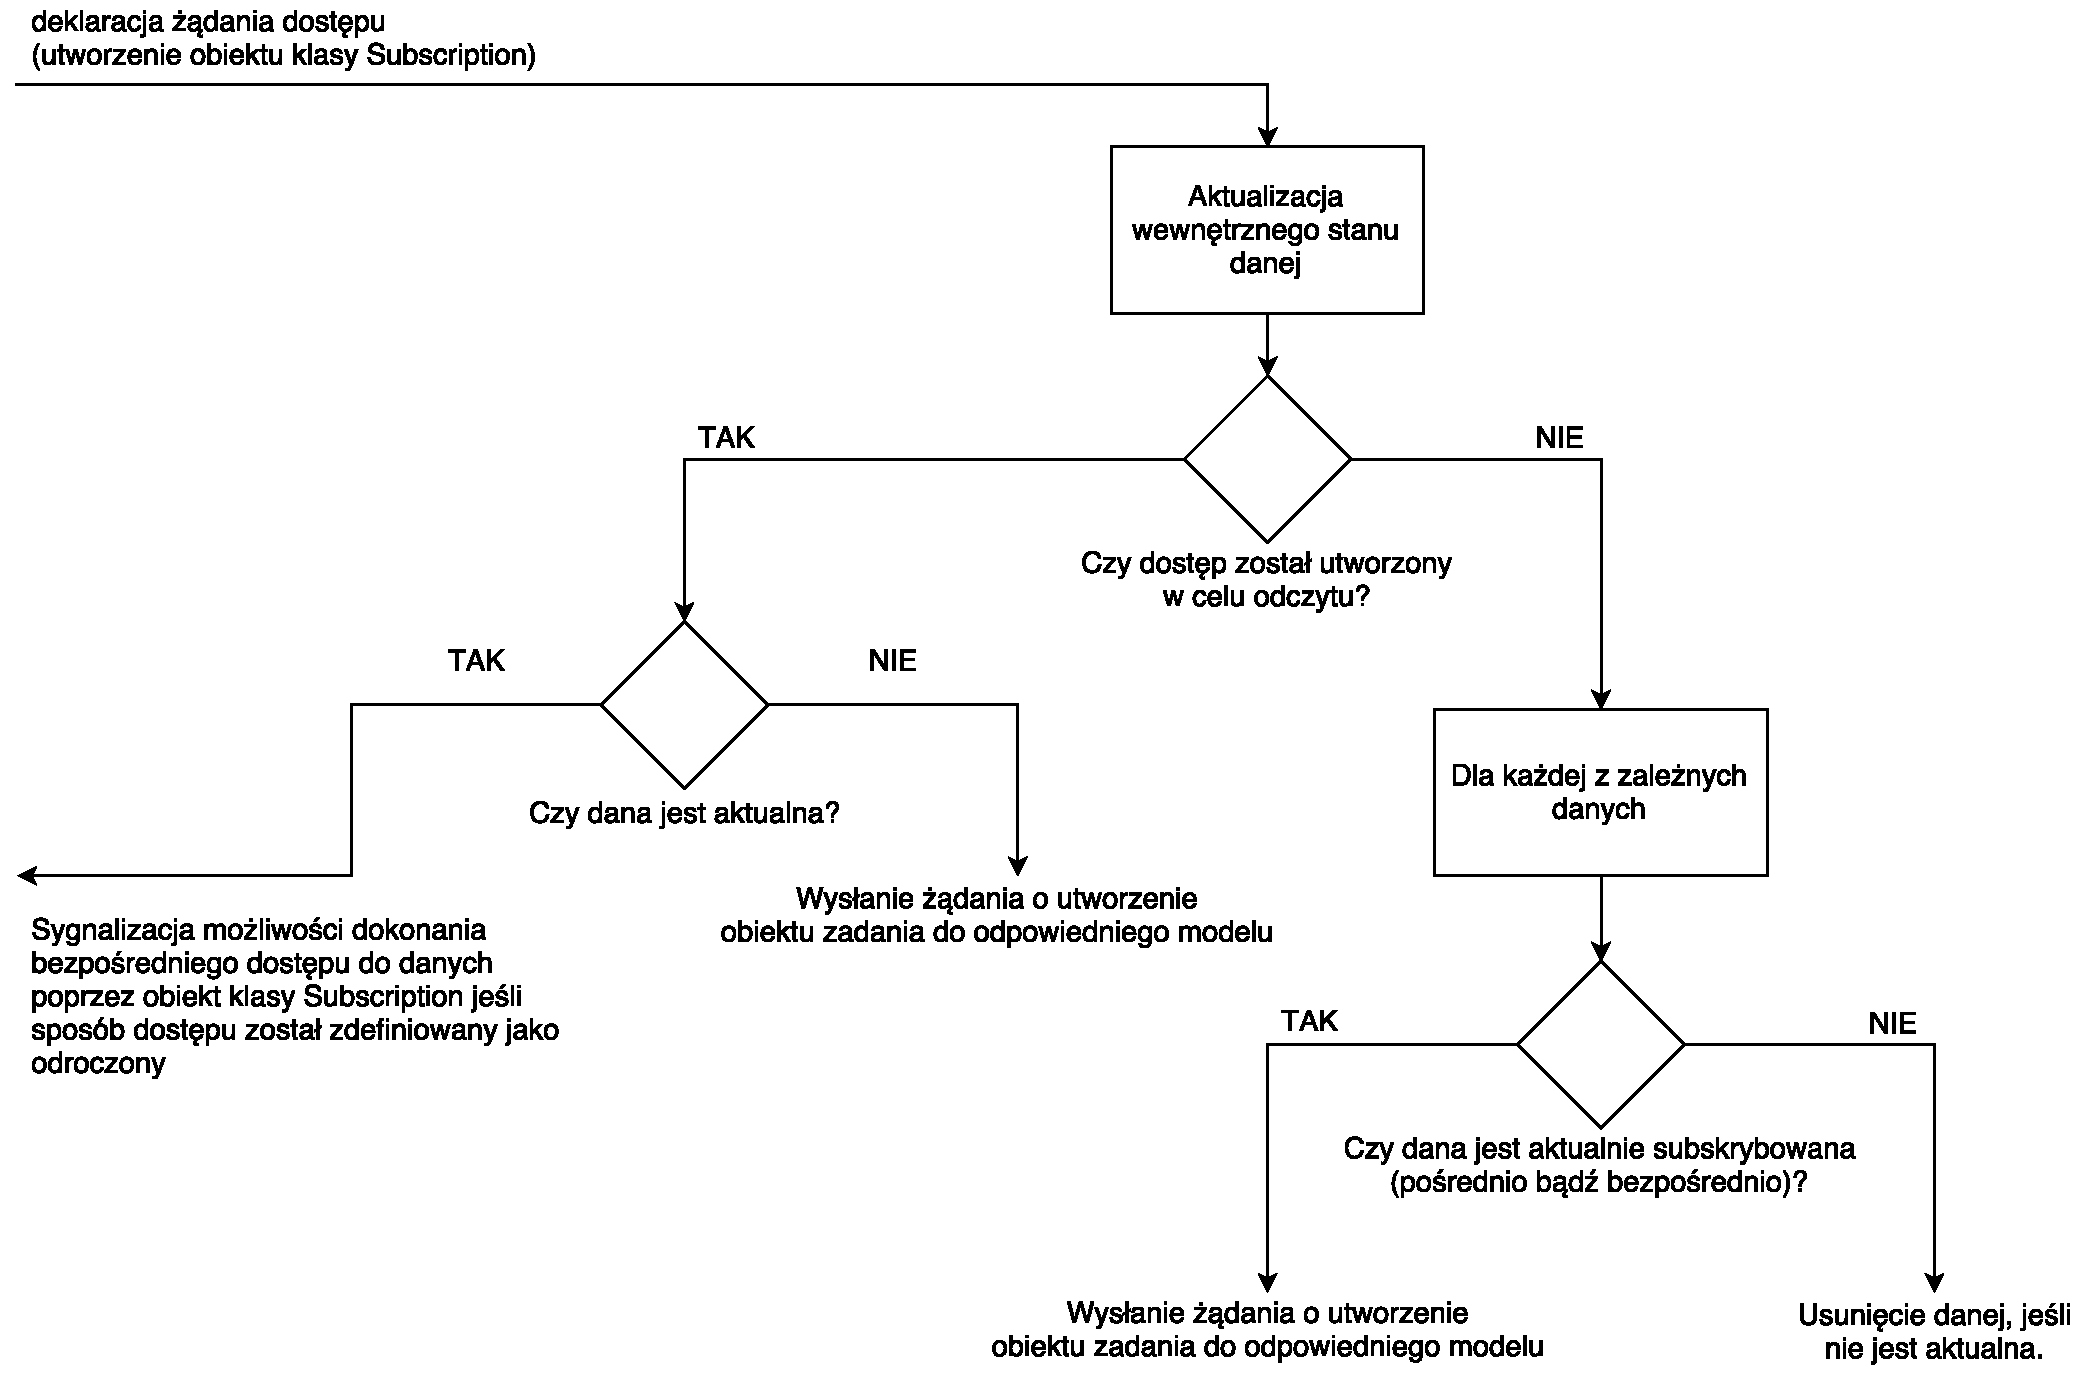
\includegraphics[width=1\linewidth]{rys05/subscribe}
	\caption{Schemat działania podczas rejestrowania faktu subskrypcji.}
	\label{fig:subscribe}	
\end{figure}

Klasa \lstinline$SubscriptionManager$ musi podjąć również jakąś akcję w~przypadku, gdy obiekt klasy \lstinline$Subscription$ zostanie usunięty. Kolekcja tych obiektów zostaje wówczas zaktualizowana. Jeżeli kolekcja ta jest pusta, dana oraz metadana zostają zwolnione, a~flagom inicjalizacji oraz aktualności zostaje przypisany fałsz.
Jeżeli kolekcja nie jest pusta, wówczas jeśli sytuacja odnosiła się do obiektu klasy \lstinline$Subscription$ utworzonego w~celu odczytu dodatkowo zostaje dekrementowany licznik takich obiektów, zaś w~przypadku obiektu klasy \lstinline$Susbscription$ utworzonego w~celu zapisu/modyfikacji, fladze wskazującej na istnienie takiego obiektu zostaje przypisany fałsz, a~do wszystkich subskrybentów (komponentów posiadających obiekty klasy \lstinline$Subscription$ zdefiniowane z~odroczonym sposobem dostępu) danej zostaje wysłany sygnał o~aktualizacji danej. Scenariusz ten został przedstawiony na rysunku \ref{fig:unsubscribe}.

\begin{figure}[ht]
	\centering
	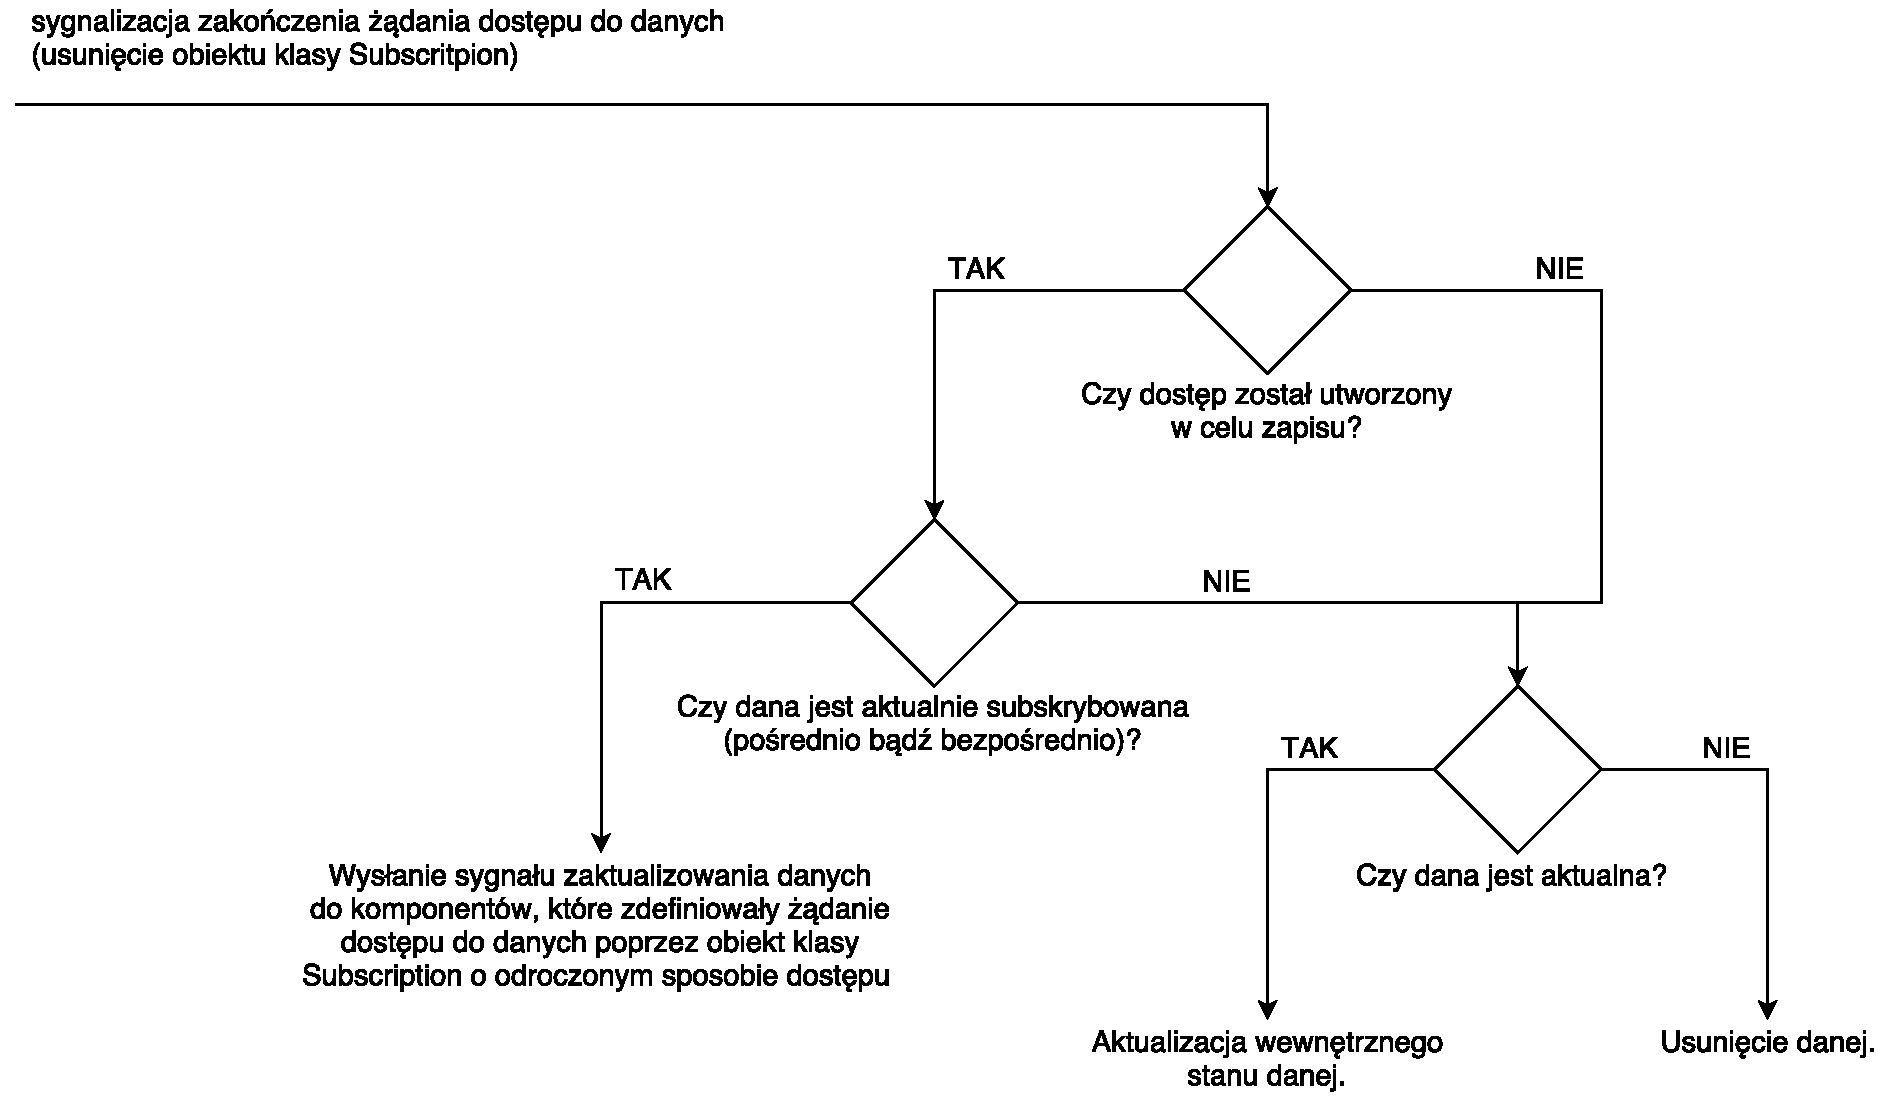
\includegraphics[width=1\linewidth]{rys05/unsubscribe}
	\caption{Schemat działania podczas usuwania subskrypcji.}
	\label{fig:unsubscribe}	
\end{figure}

Gdy ma miejsce faktyczny dostęp do danych, poprzez obiekt klasy \lstinline$Lock$, w~celu odczytu obiekt klasy \lstinline$SubscriptionManager$ wywołuje metodę \lstinline$read$ klasy \lstinline$DataEntry$, inkrementuje licznik aktywnych dostępów do danych w~celu odczytu oraz zwraca dane pozyskane za pomocą metody. Podczas dostępu w~celu zapisu sytuacja jest analogiczna -- jedyną różnicą jest fakt przypisania wartości prawdy fladze aktywnego dostępu zamiast inkrementacji licznika. 

Gdy faktyczny dostęp w~celu odczytu zostaje zakończony wywołana zostaje metoda \lstinline$endRead$ klasy \lstinline$DataEntry$, a~licznik aktywnych dostępów zostaje dekrementowany. W~sytuacji zakończenia zapisu wywoływana zostaje metoda \lstinline$endWrite$, flaga wskazująca na aktywny zapis zostaje ustawiona na fałsz, a~flagom wskazującym zainicjalizowanie oraz aktualność danej przypisana jest prawda.

\section{Porównanie systemów}
Przewagę nowego systemu zarządzania danymi oraz procesem wykonania można wyróżnić na 2 płaszczyznach -- dostępu do danych współdzielonych oraz zapewnienia propagacji sygnałów aktualizacji danych.

\subsection{Dostęp do danych współdzielonych}

Bezpieczeństwo dostępu do danych zostało poprawione w~nowej wersji systemu.


\begin{minipage}{\textwidth}
	\begin{lstlisting}[label=dataaccess:old, caption={Przykład dostępu do danych według bieżącego systemu.},alsoletter={()[].=}]
	SharedDataLock ctxlock(ctx->mutex);
	limiters.assign((*ctx)->dimensionality, std::make_pair(0, (*ctx)->nbins-1));
	\end{lstlisting}
\end{minipage}

Na listingu \ref{dataaccess:old} przedstawiony został sposób dostępu do danych współdzielonych w~obecnej architekturze. Z~analizy listingu wynika, że przed faktycznym dostępem do danych wykonywane jest zajęcie muteksu skojarzonego z~tą daną. Pozostawienie odpowiedzialności synchronizacji dostępu programiście, który chce ich użyć jest zabiegiem niebezpiecznym. Programista może kwestię synchronizacji pominąć, lub o~niej zapomnieć. Skutkować to może naruszeniem ochrony pamięci i~zakończeniem działania programu.

\begin{minipage}{\textwidth}
	\begin{lstlisting}[label=dataaccess:new, caption={Przykład dostępu do danych według nowego systemu.},alsoletter={()[].=}]
	Subscription::Lock<multi_img> lock(*sub);
	multi_img* img = lock();
	QPixmap pix = QPixmap::fromImage(img->export_qt(1));
	\end{lstlisting}
\end{minipage}

Na listingu \ref{dataaccess:new} został przedstawiony sposób dostępu do danych współdzielonych za pomocą nowego systemu. Z analizy listingu można wywnioskować, że w~tym systemie programista, który chce użyć danych nie jest zobowiązany do wykonywania synchronizacji dostępu. Rzecz ta należy do funkcjonalności modelu danych współdzielonych i~wykonywana jest automatycznie podczas żądania dostępu.

\subsection{Propagacja sygnałów aktualizacji danych}

Sposób definiowania procesu wykonania danych uległ diametralnej zmianie. Obecny system zarządzania procesem wykonania jest zdecentralizowany. Aby utworzenie danej~A było zlecone na skutek obliczenia danej~B, model~B musi emitować sygnał informujący o~obliczeniu danej~B, model~A posiadać slot w~którym zdefiniowana jest reakcja na taki sygnał oraz kontroler (jako element warstwy nadrzędnej) musi ustanowić połączenie pomiędzy danym sygnałem i~slotem. W~wyniku tego aby zapewnić odpowiedni proces wykonania w~systemie, należy ręcznie ustanowić bardzo wiele połączeń, co zaciemnia kod. Przykład takiego zaciemnienia może stanowić listing \ref{propagation:old}.

\begin{minipage}{\textwidth}
	\begin{lstlisting}[label=propagation:old, caption={Przykład definiowania procesu wykonania według starego systemu.},alsoletter={()[].=}]
	connect(lm, SIGNAL(newLabeling(const cv::Mat1s&, const QVector<QColor>&, bool)), dvc, SLOT(updateLabels(cv::Mat1s,QVector<QColor>,bool)));
	connect(lm, SIGNAL(partialLabelUpdate(const cv::Mat1s&,const cv::Mat1b&)), dvc, SLOT(updateLabelsPartially(const cv::Mat1s&,const cv::Mat1b&)));
	connect(dvc, SIGNAL(alterLabelRequested(short,cv::Mat1b,bool)), lm, SLOT(alterLabel(short,cv::Mat1b,bool)));
	connect(illumm, SIGNAL(newIlluminantCurve(QVector<multi_img::Value>)), dvc, SIGNAL(newIlluminantCurve(QVector<multi_img::Value>)));
	connect(illumm, SIGNAL(newIlluminantApplied(QVector<multi_img::Value>)), dvc, SIGNAL(newIlluminantApplied(QVector<multi_img::Value>)));
	\end{lstlisting}
\end{minipage}

W nowym systemie definiowana procesu wykonania problem ten nie istnieje. Proces wykonania jest definiowany przez deklaracje danych współdzielonych i~ich zależności, natomiast klasa \lstinline$SubscriptionManager$ zapewnia funkcjonalność informowania modeli o~potrzebie utworzenia zadania przetwarzającego dane. W~związku z~tym w~nowej architekturze systemu nie istnieje potrzeba aby ręcznie zarządzać procesem przetworzenia danych.

